\chapter{Проектирование и реализация инфраструктуры программных системы для работы с большими данными} \label{ch4}

% не рекомендуется использовать отдельную section <<введение>> после лета 2020 года
%\section{Введение} \label{ch4:intro}

% Хорошим стилем является наличие введения к главе. Во введении может быть описана цель написания главы, а также приведена краткая структура главы. 
Весь процесс проектирования можно иллюстрировать следующей диаграммой активности (\firef{fig:diagram_activity})

\begin{figure}
  \center
  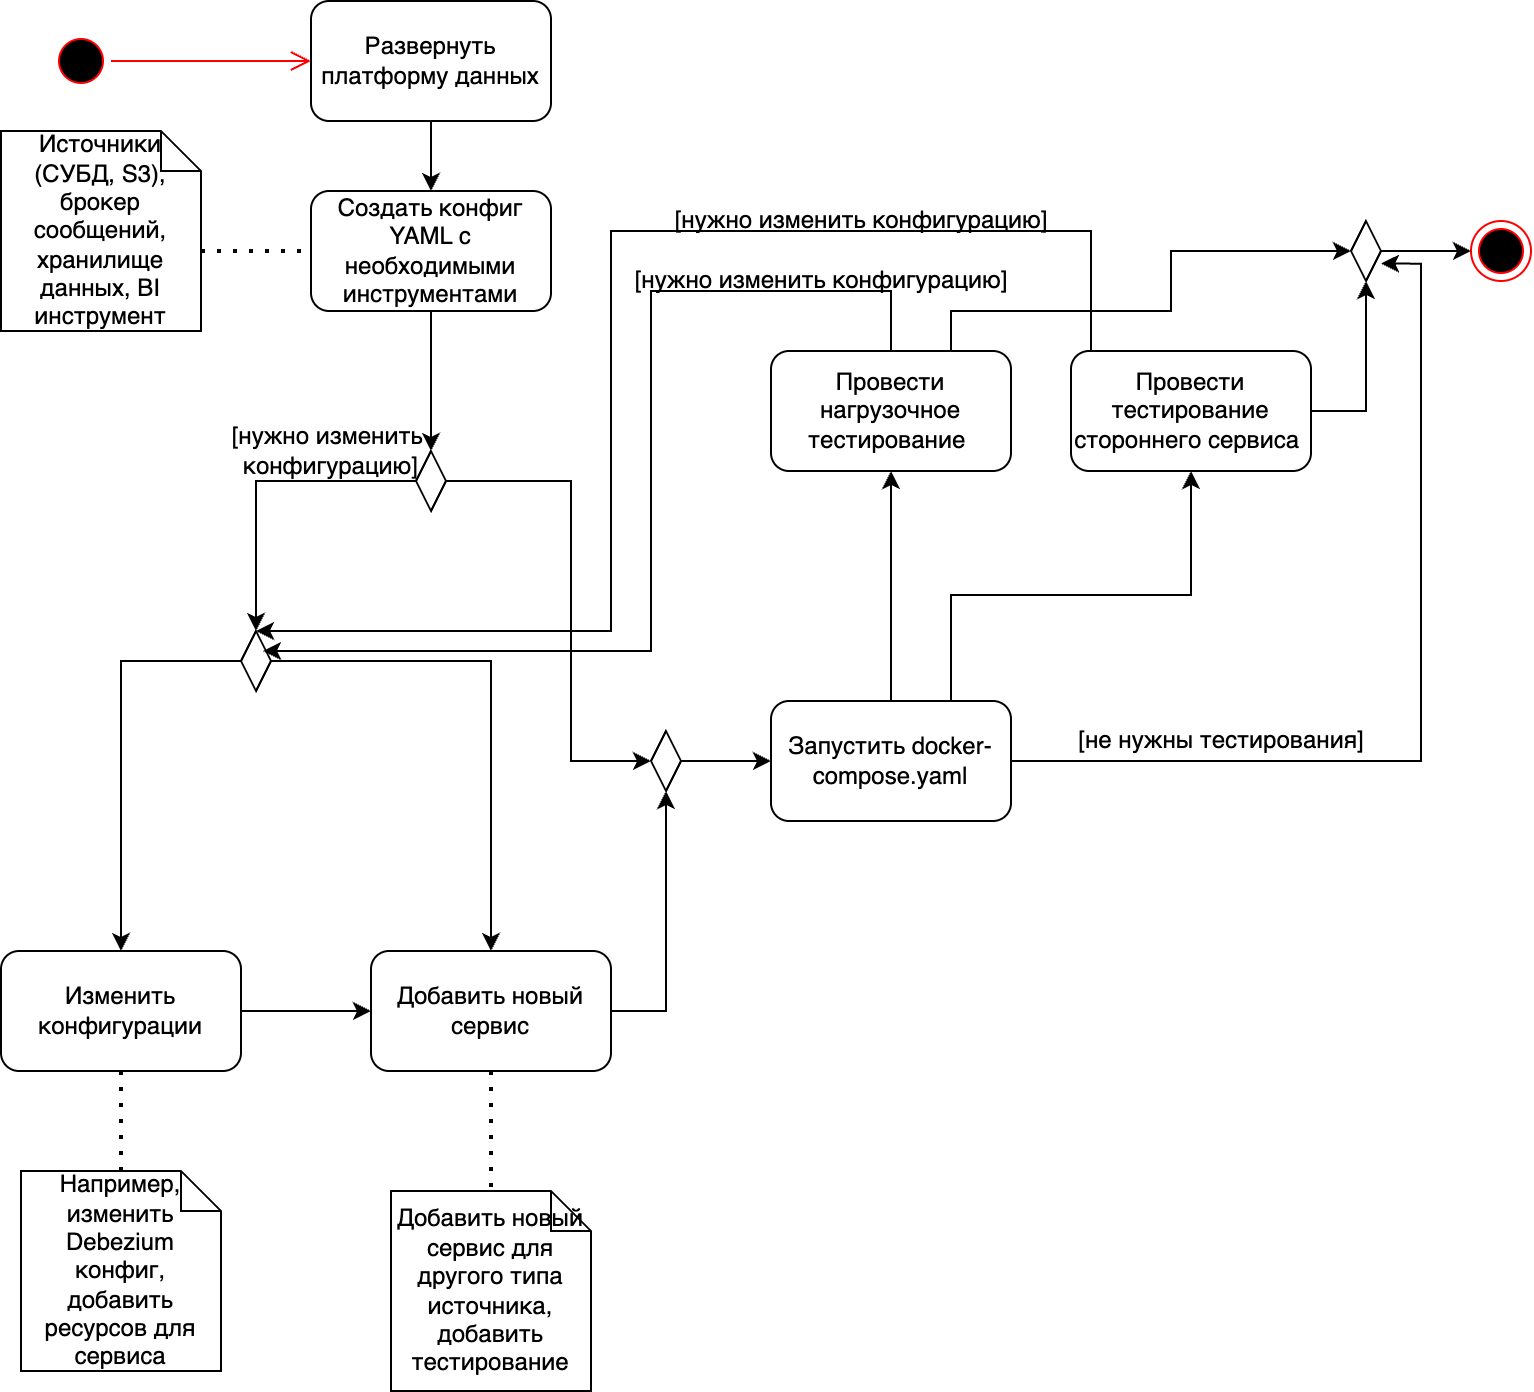
\includegraphics [scale=0.3] {my_folder/images/diagram_activity}
  \caption{Диаграмма деятельности}
  \label{fig:diagram_activity}
\end{figure}
\FloatBarrier
В данном разделе будут рассмотрены практические примеры использования инструмента для развертывания полноценных платформ данных. На примере двух известных датасетов, Northwind\cite{northwind} и Chinook\cite{chinook}, будет продемонстрирован весь цикл настройки и работы конвейера данных: от источников до систем хранения и визуализации. Эти примеры иллюстрируют, как с помощью декларативной конфигурации можно быстро построить и запустить сложную инфраструктуру для анализа данных.



\section{Пример Northwind: Связь клиентов с заказами} \label{ch4:northwind}
Данный пример демонстрирует полный цикл обработки данных с использованием платформы, сгенерированной инструментом dpd на основе простой конфигурации. В качестве источника используется классический датасет "Northwind"\cite{northwind}, загруженный в СУБД PostgreSQL.

Цель – показать, как данные из операционной базы данных проходят через систему потоковой обработки Kafka, сохраняются в аналитическом хранилище ClickHouse и визуализируются с помощью BI-инструмента Superset. Параллельно данные также архивируются в S3-совместимое хранилище Minio.

\begin{enumerate}[1.]
  \item Конфигурация платформы\\
        Для генерации инфраструктуры использовался следующий конфигурационный файл \texttt{config.yaml}:
        \begin{verbatim}
project:
  name: data-platform-northwind 
  version: 1.0.0
  description: Northwind end-to-end
sources:
  - type: postgres
    name: postgres_1
  - type: postgres
    name: postgres_2 # Дополнительный источник
  - type: s3
    name: s3_1      # S3-совместимое хранилище (Minio)
streaming:
  kafka:
    num_brokers: 6
  connect:
    name: connect-1 
storage:
  clickhouse:
    name: clickhouse-1 # Аналитическое хранилище
bi:
  superset:
    name: superset-1 # BI-инструмент  
\end{verbatim}

  \item Развертывание и статус сервисов\\
        После запуска команды \texttt{dpd generate ---config config.yaml} был создан файл \texttt{docker-compose.yml} и сопутствующие конфигурации. Платформа была развернута стандартной командой \texttt{docker compose up -d}. Все сервисы (PostgreSQL, Minio, Kafka-брокеры, Kafka Connect, Kafka UI, ClickHouse, Superset) успешно запустились и работали в штатном режиме(\firef{fig:ex1_docker_services}).
        \clearpage
        \begin{figure}[h]
          \center
          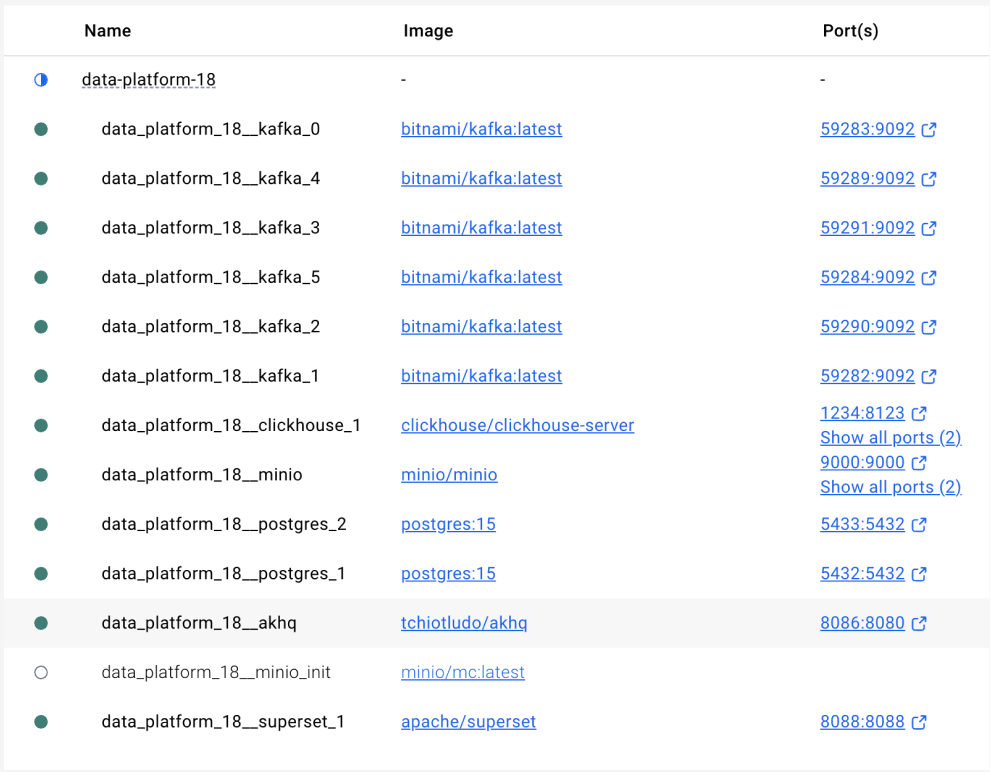
\includegraphics [scale=0.4] {my_folder/images/ex1_docker_services.png}
          \caption{ Статус сервисов в Docker Desktop}
          \label{fig:ex1_docker_services}
        \end{figure}
        \clearpage
        \FloatBarrier
  \item Поток данных от источника до BI
        \begin{itemize}
          \item Источник данных (PostgreSQL)\\
                База данных Northwind была предварительно загружена в экземпляр PostgreSQL. DDL базы Northwind изображена на рисунке \ref{fig:ex1_schema_ddl}
                \begin{figure}
                  \center
                  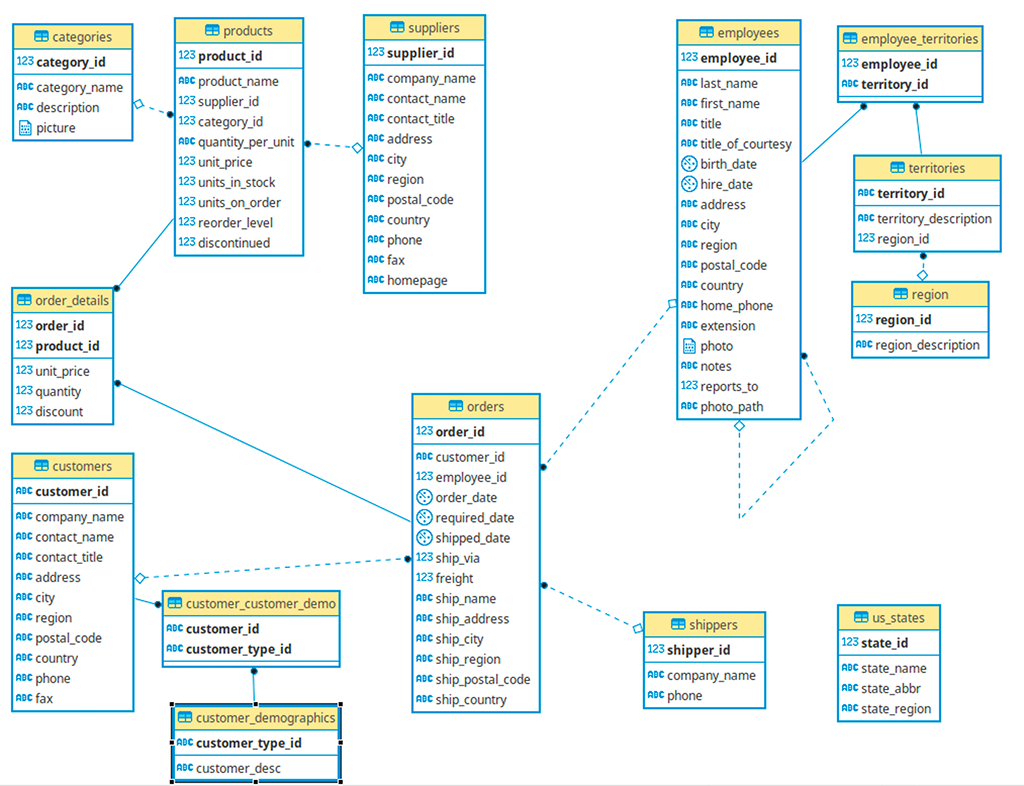
\includegraphics [scale=0.8] {my_folder/images/ex1_schema_ddl}
                  \caption{DDL схемы Northwind в PostgreSQL}
                  \label{fig:ex1_schema_ddl}
                \end{figure}
                \FloatBarrier
          \item Захват изменений (Debezium + Kafka Connect):\\
                Для отслеживания изменений (операций INSERT, UPDATE, DELETE) в таблицах PostgreSQL были автоматически созданные коннекторы Debezium PostgreSQL и S3SinkSourceConnector, работающий внутри сервиса Kafka Connect. Коннектор читает WAL (Write-Ahead Log) базы данных и публикует все изменения в виде сообщений в соответствующие топики Apache Kafka. Для каждой таблицы был автоматически создан свой топик.
                \begin{figure}
                  \center
                  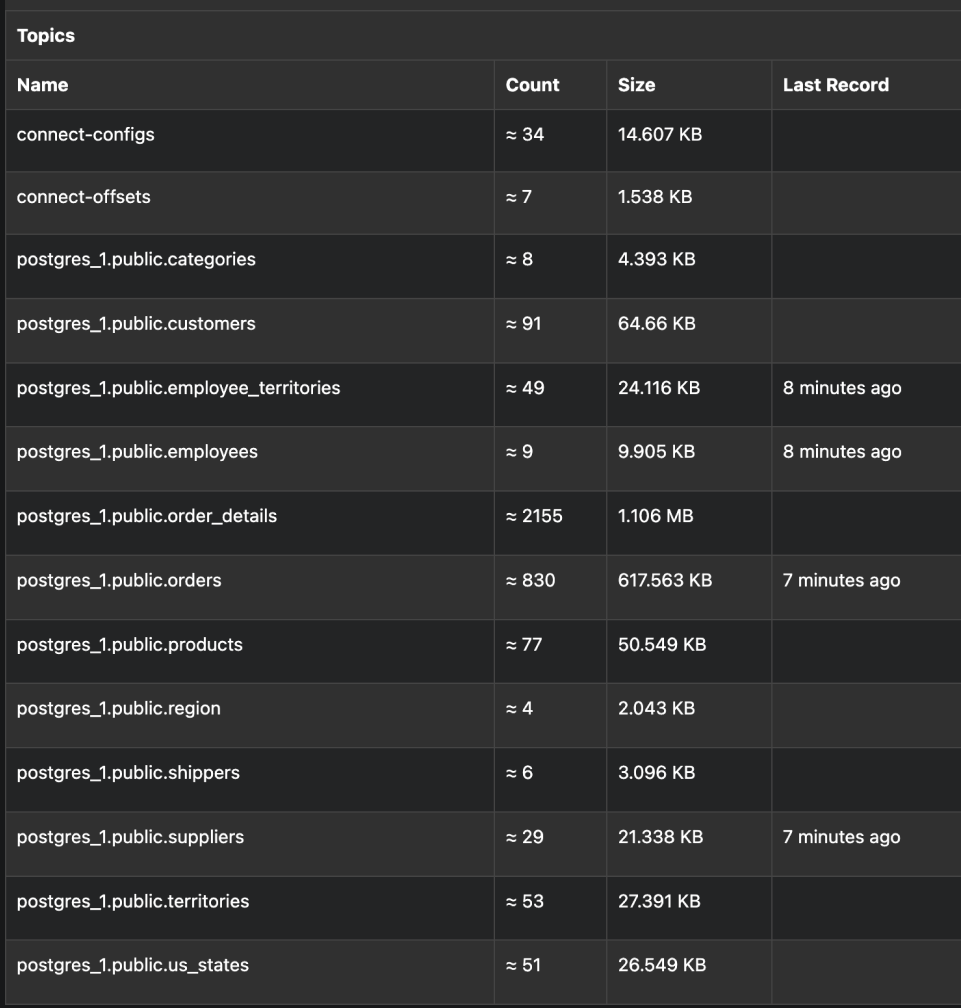
\includegraphics [scale=0.3] {my_folder/images/ex1_kafka_topics}
                  \caption{Список активных Kafka-топиков в Kafka UI}
                  \label{fig:ex1_kafka_topics}
                \end{figure}
                \FloatBarrier
                \begin{figure}
                  \center
                  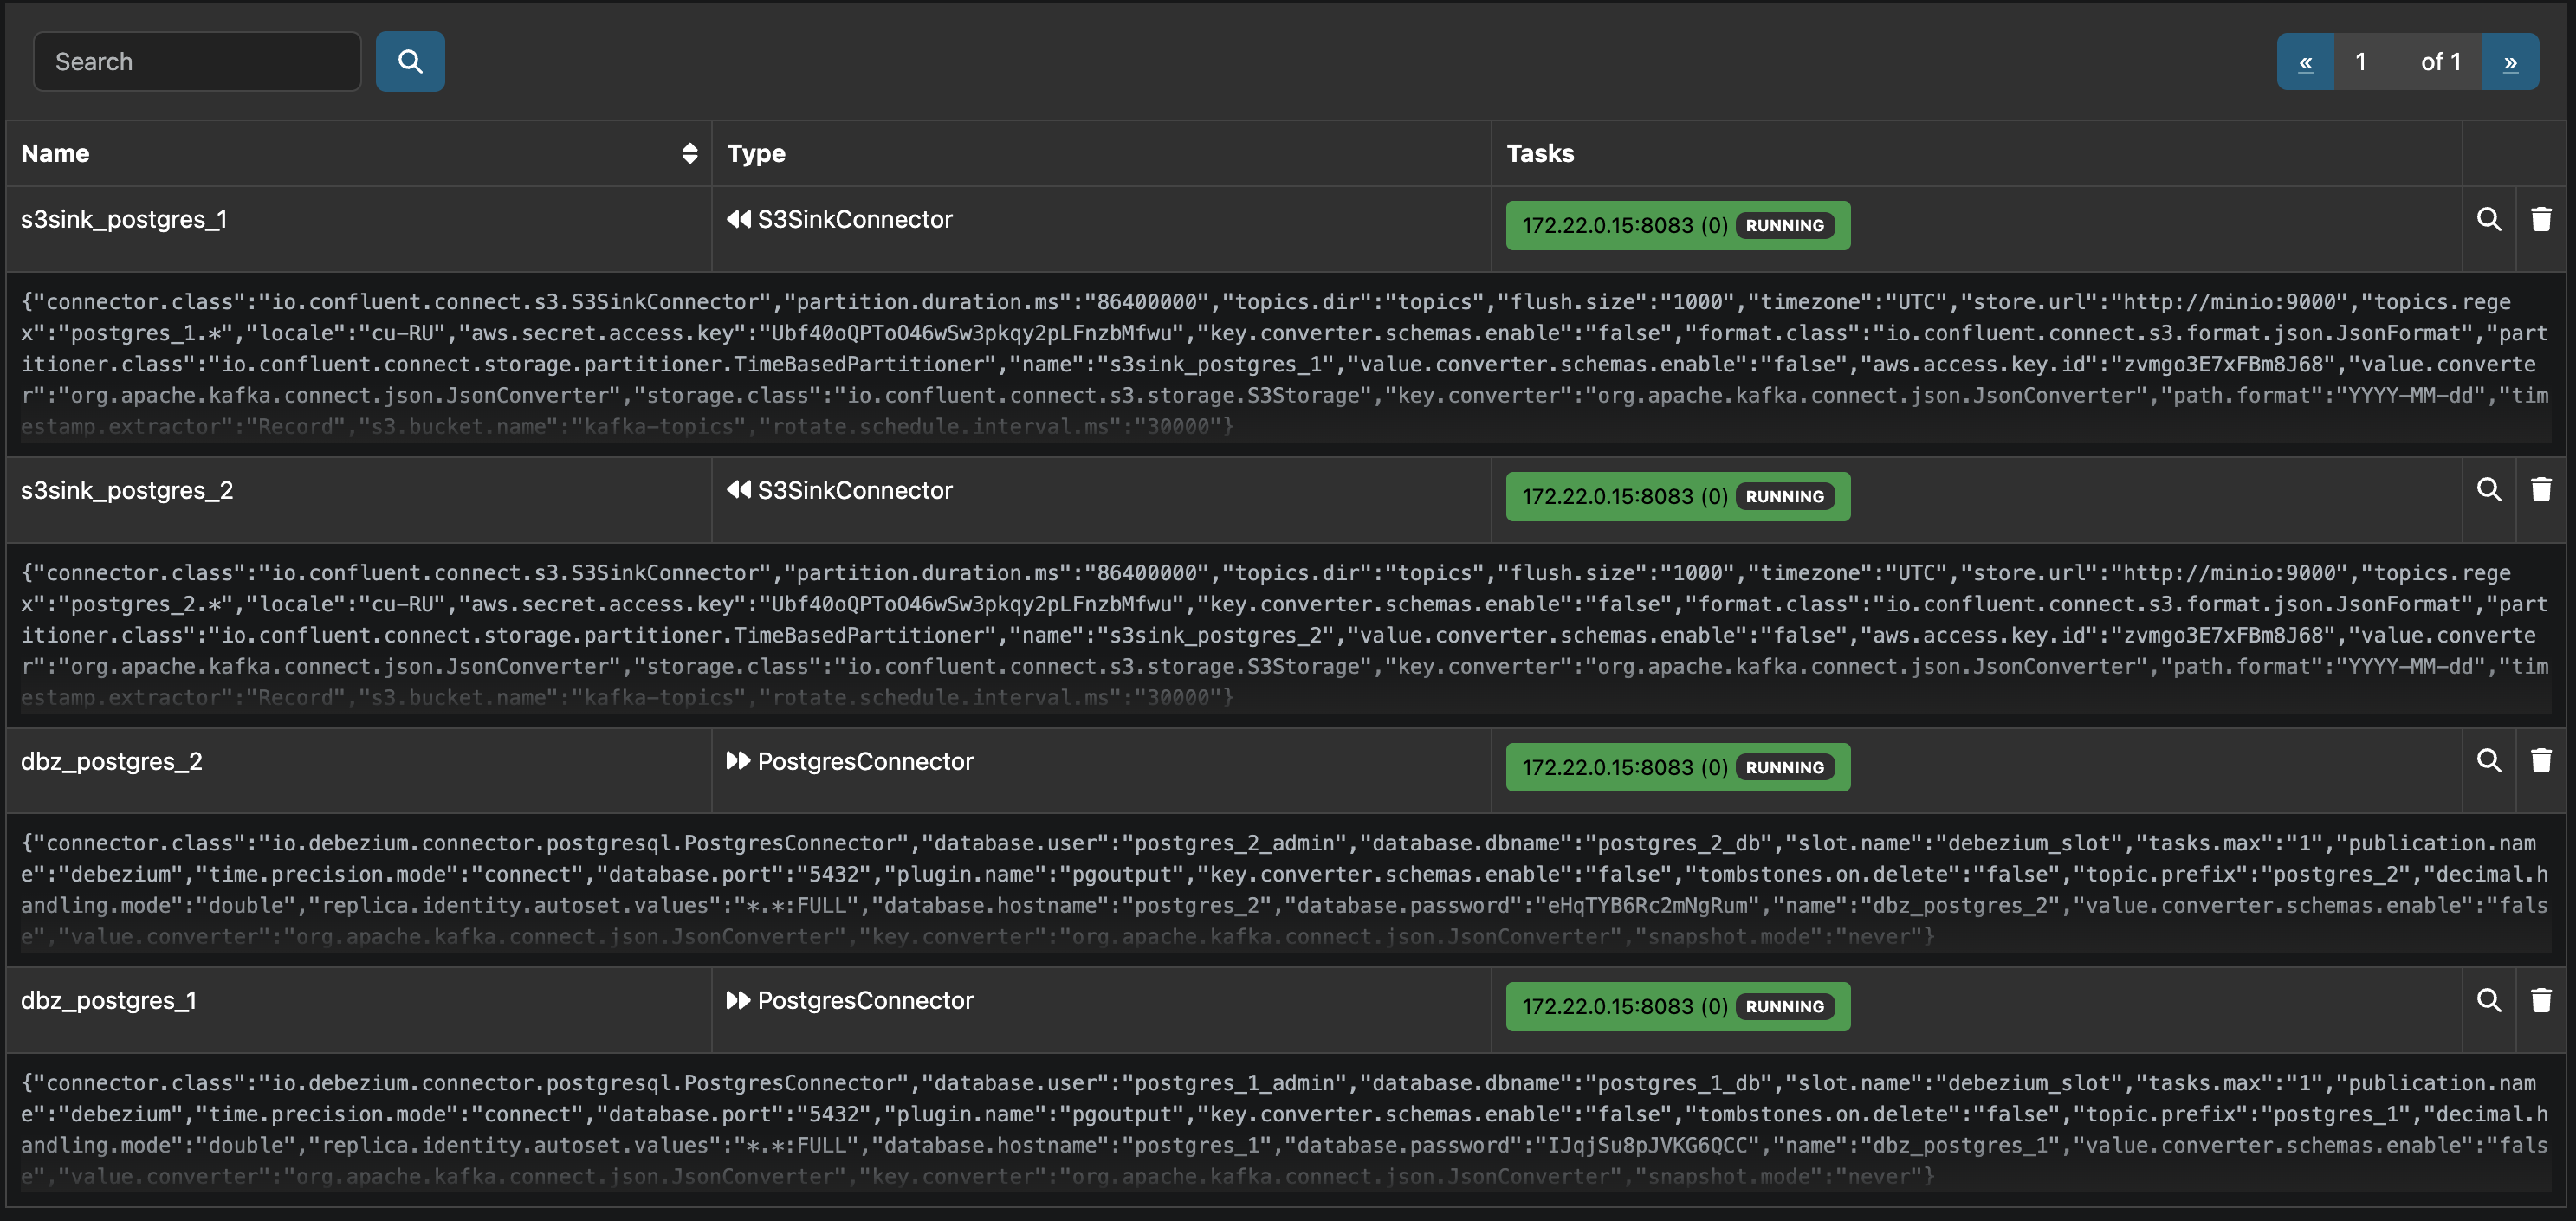
\includegraphics [scale=0.3] {my_folder/images/ex1_kafka_connectors}
                  \caption{Коннекторы в Kafka UI}
                  \label{fig:ex1_kafka_connectors}
                \end{figure}
                \FloatBarrier
          \item Загрузка в аналитическое хранилище (ClickHouse):\\
                Данные из Kafka доставлялись в ClickHouse с использованием встроенного движка KafkaEngine. Для каждой таблицы источника была создана связка:
                \begin{enumerate}[1.]
                  \item Таблица на движке KafkaEngine\cite{clickhouse}, которая подписывается на соответствующий топик Kafka и читает из него сообщения "на лету".
                  \item Целевая таблица на движке MergeTree\cite{clickhouse} для эффективного хранения и аналитических запросов.
                  \item Материализованное представление, которое автоматически считывает данные из Kafka-таблицы и вставляет их в MergeTree-таблицу, выполняя при необходимости базовые преобразования.
                \end{enumerate}
                Пример SQL кода для забора данных из Kafka в ClickHouse для таблицы \texttt{orders} находится в приложении \ref{ex_1_sql}
                \begin{figure}
                  \center
                  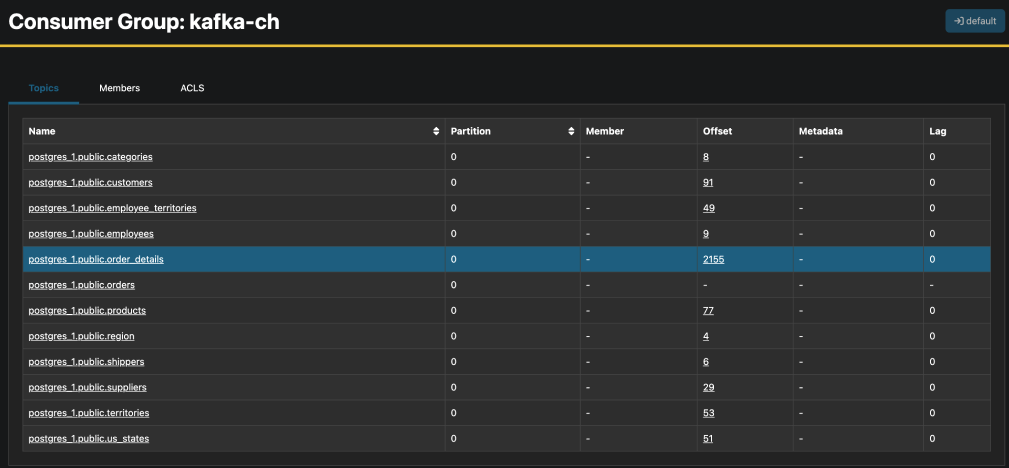
\includegraphics [scale=0.45] {my_folder/images/ex1_kafka_ch_consumer}
                  \caption{Группы консьюмеров ClickHouse в Kafka UI}
                  \label{fig:ex1_kafka_ch_consumer}
                \end{figure}
                \FloatBarrier
          \item Архивация данных в S3\\
                Параллельно с основной обработкой, данные из Kafka-топиков архивировались
                в S3-хранилище (реализованное через Minio). Kafka Connect S3 Sink Connector считывал сообщения
                из топиков и сохранял их в виде файлов JSON в соответствующие директории внутри S3 бакета(рис \ref{fig:ex1_s3}). Это обеспечивает долговременное хранение сырых данных.
                \begin{figure}
                  \center
                  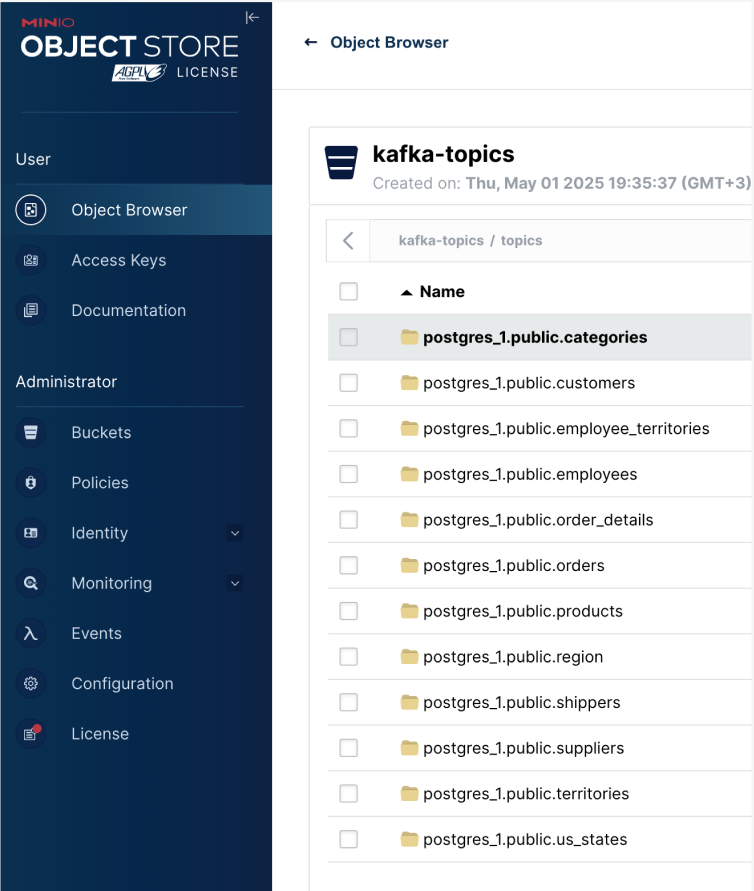
\includegraphics [scale=0.45] {my_folder/images/ex1_s3}
                  \caption{ Список директорий в S3, соответствующих топикам Kafka}
                  \label{fig:ex1_s3}
                \end{figure}
                \FloatBarrier
          \item Загрузка и хранение в ClickHouse\\
                Данные о продажах и связанных сущностях доставлялись из Kafka в ClickHouse с использованием стандартного паттерна c предыдущего примера: Kafka Engine таблица для чтения из топика и Materialized View для переноса данных в целевую таблицу на движке MergeTree. Это позволило эффективно хранить данные для аналитических запросов.
          \item Проверка целостности данных\\
                Было проведено сравнение количества записей в ключевых таблицах источника (PostgreSQL) и приемника (ClickHouse). Сравнение показало полное совпадение количества строк, что свидетельствует об успешной и полной доставке данных.
                \begin{figure}
                  \center
                  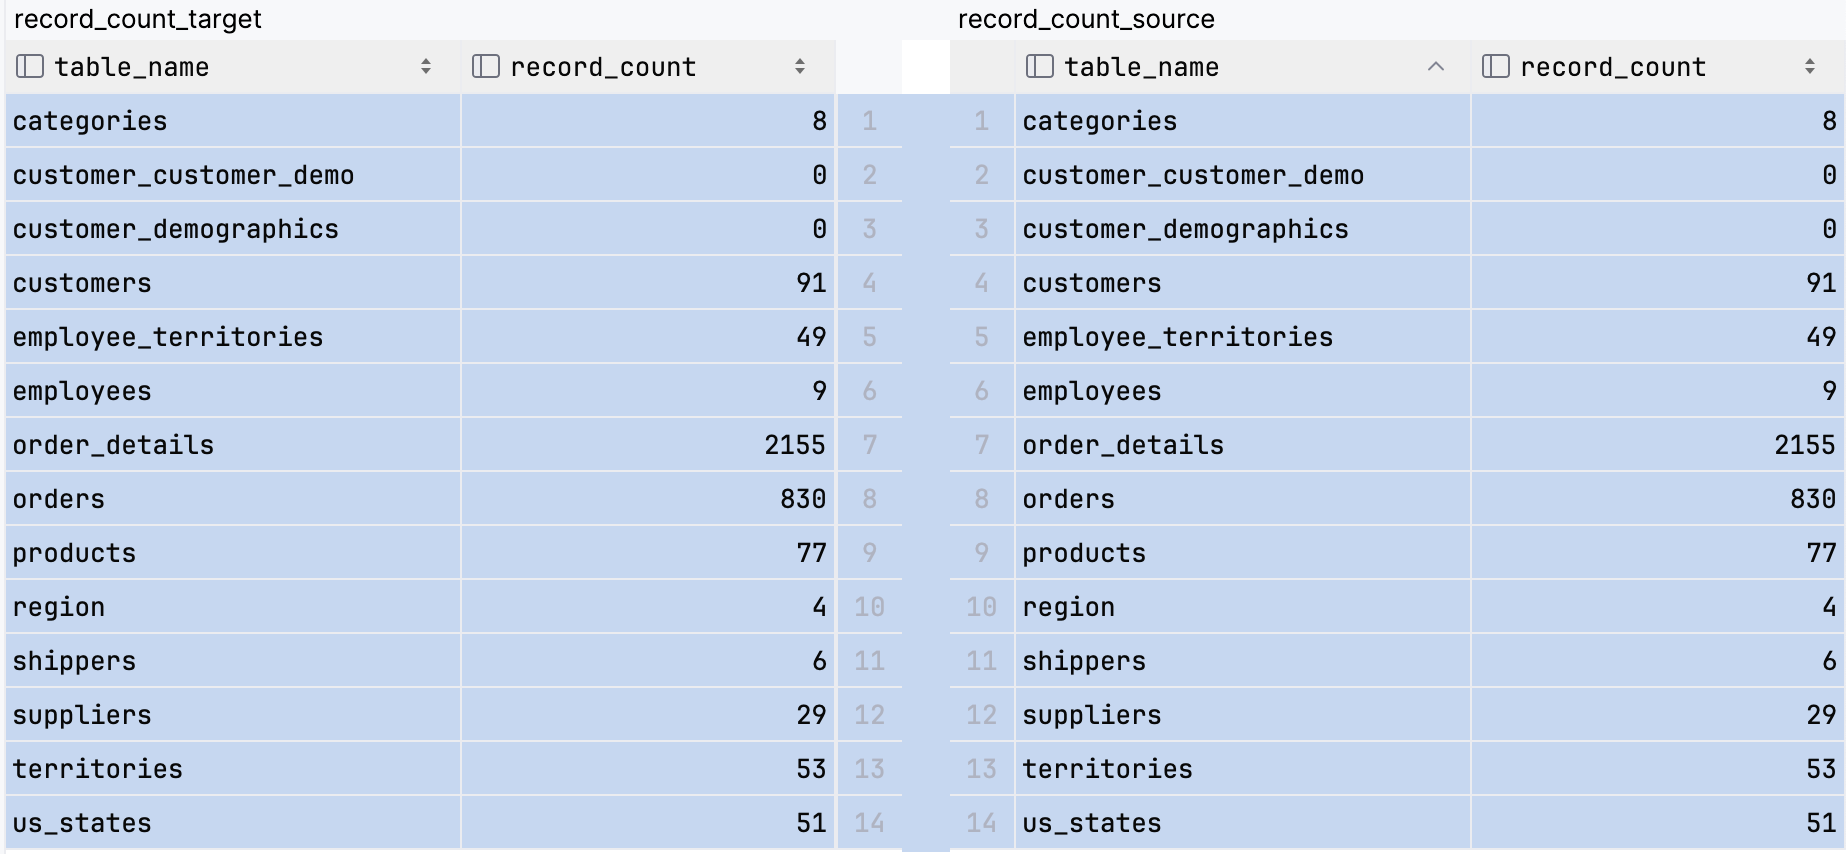
\includegraphics [scale=0.5] {my_folder/images/ex1_tables_ch_pg_compraring}
                  \caption{Сравнение количества строк в PostgreSQL и ClickHouse для Northwind}
                  \label{fig:ex1_tables_ch_pg_compraring}
                \end{figure}
                \FloatBarrier
          \item Анализ и Визуализация (Superset)\\
                Данные, загруженные в ClickHouse, были подключены как источник в Apache Superset. На основе этих данных был построен дашборд, включающий визуализацию, например, график среднего времени обработки заказа по месяцам(\firef{fig:ex1_superset_chart}). Это демонстрирует готовность данных к анализу и построению отчетности.
                \begin{figure}
                  \center
                  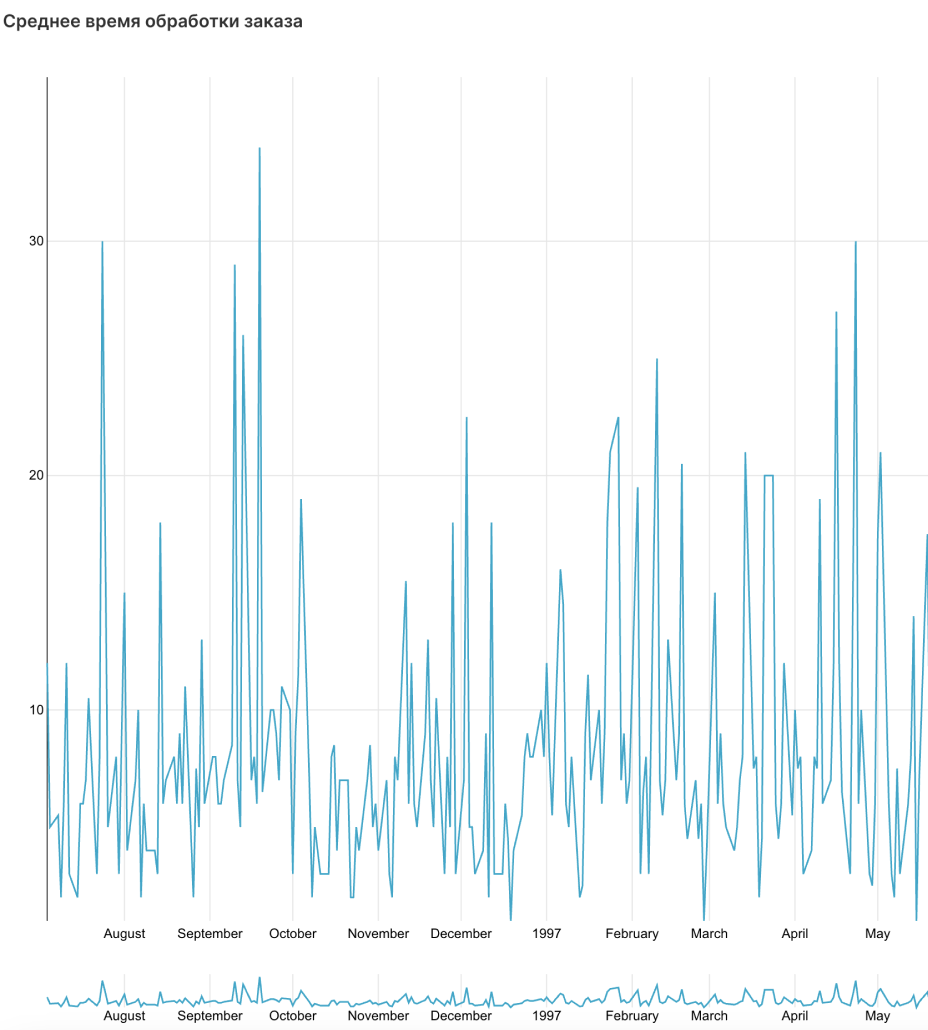
\includegraphics [scale=0.45] {my_folder/images/ex1_superset_chart}
                  \caption{Чарт в Superset "Среднее время обработки заказа"}
                  \label{fig:ex1_superset_chart}
                \end{figure}
                \FloatBarrier


        \end{itemize}
\end{enumerate}
\FloatBarrier
Данный пример успешно продемонстрировал возможность быстрого развертывания комплексной платформы данных с использованием инструмента автоматической генерации платформы данных и одного конфигурационного файла. Был реализован сквозной data pipeline: от захвата изменений в реляционной БД, через потоковую обработку в Kafka, с параллельной выгрузкой в S3, до загрузки в аналитическое хранилище ClickHouse и последующей визуализации в Superset. Проверка целостности данных подтвердила корректность работы всех компонентов пайплайна.

\clearpage
\FloatBarrier
\section{Пример Chinook: Анализ музыкальных продаж } \label{ch4:ex_chinhook}

Второй пример демонстрирует применение нашего инструмента для построения аналитического конвейера на основе датасета "Chinook"\cite{chinook}, который моделирует базу данных цифрового музыкального магазина. Цель — отследить поток данных о продажах от операционной базы данных через Kafka до аналитического хранилища ClickHouse и S3-архива, с последующей визуализацией ключевых метрик в Superset.

\begin{enumerate}[1.]
  \item Конфигурация платформы\\
        Для генерации инфраструктуры под этот сценарий использовался аналогичный по структуре конфигурационный файл, адаптированный под новый проект и источники:
        \begin{verbatim}
project:
  name: chinehook
  version: 1.0.0
  description: This is a project for chinook
sources:
  - type: postgres
    name: postgres_chinook
  - type: postgres
    name: postgres_2
  - type: s3
    name: s3_1
streaming:
  kafka:
    num_brokers: 6
  connect:
    name: connect-1
storage:
  clickhouse:
    name: clickhouse-1 
bi:
  superset:
    name: superset-1
    \end{verbatim}
  \item{Развертывание платформы}\\
        Аналогично первому примеру, команда \texttt{dpd generate --config config-chinook.yaml} создала необходимый \texttt{docker-compose.yml} и конфигурационные файлы. Запуск \texttt{docker compose up -d} успешно развернул все компоненты платформы.
  \item{Поток данных и артефакты}
        \begin{itemize}
          \item Источник данных (PostgreSQL)\
                База данных Chinook, DDL которой изображена на рисунке \ref{fig:ex2_schema_ddl} была загружена в экземпляр PostgreSQL (\texttt{postgres\_chinook}).
                \begin{figure}[h]
                  \center
                  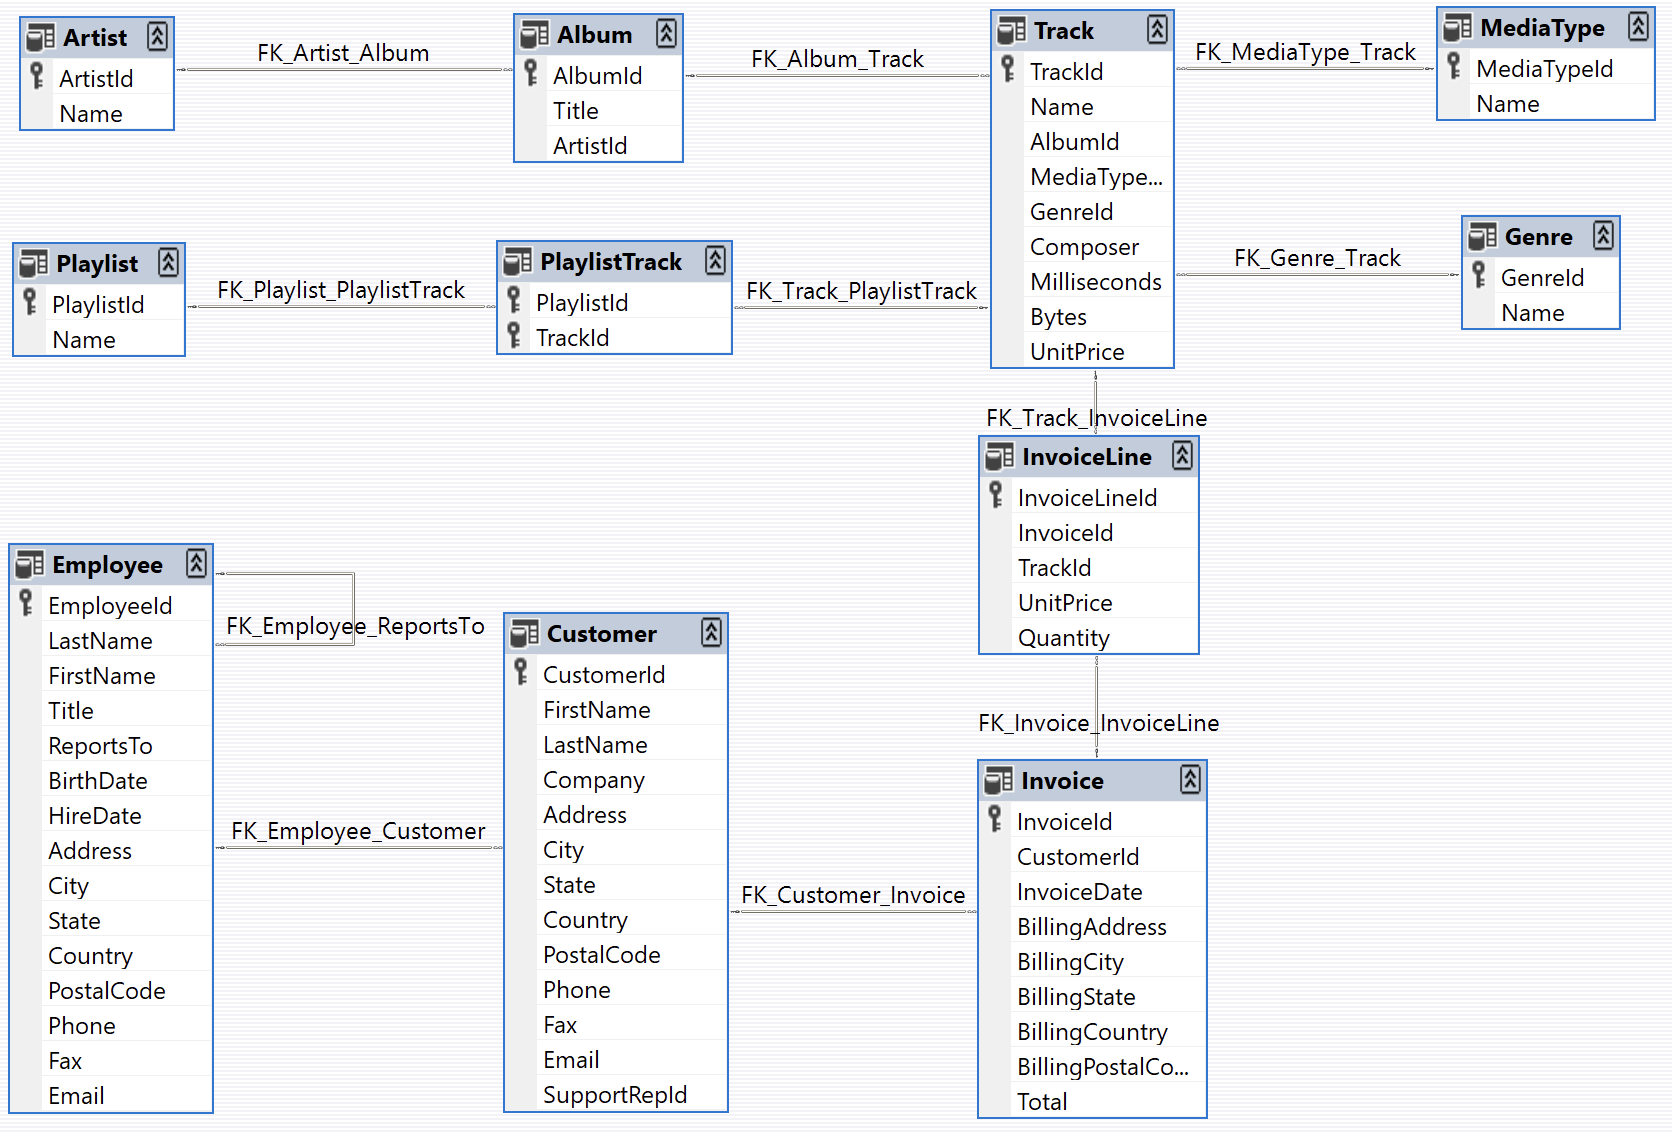
\includegraphics [scale=0.5] {my_folder/images/ex2_schema_ddl}
                  \caption{DDL схемы Chinook в PostgreSQL}
                  \label{fig:ex2_schema_ddl}
                \end{figure}
                \FloatBarrier
          \item Захват изменений и публикация в Kafka \\
                С помощью коннектора Debezium PostgreSQL, настроенного через Kafka Connect, все изменения в таблицах Chinook захватывались из WAL и публиковались в соответствующие топики Kafka(\firef{fig:ex2_kafka_topics}).
                \begin{figure}[h]
                  \center
                  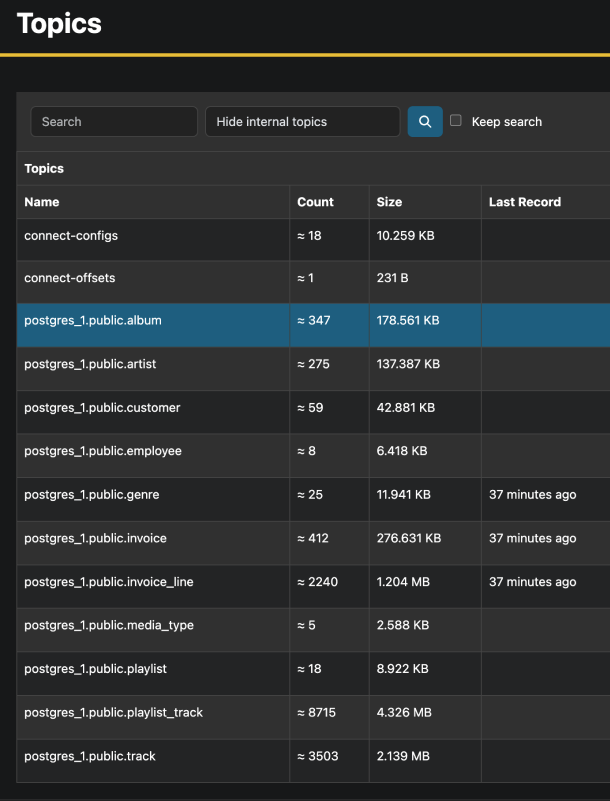
\includegraphics [scale=0.5] {my_folder/images/ex2_kafka_topics}
                  \caption{Список Kafka-топиков в Kafka UI}
                  \label{fig:ex2_kafka_topics}
                \end{figure}
                \FloatBarrier
          \item Архивация данных в S3\\
                Параллельно с основной обработкой, данные из Kafka-топиков архивировались в S3-хранилище (\firef{fig:ex2_s3}). Kafka Connect S3 Sink Connector считывал сообщения из топиков и сохранял их в виде файлов JSON в соответствующие директории внутри S3 бакета. Это обеспечивает долговременное хранение сырых данных.
                \begin{figure}[h]
                  \center
                  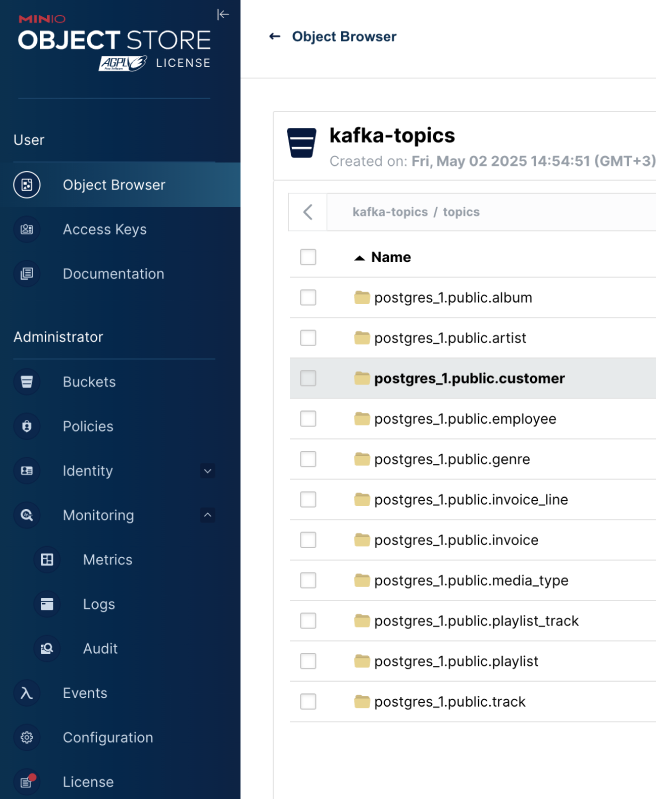
\includegraphics [scale=0.5] {my_folder/images/ex2_s3}
                  \caption{Список директорий в S3, соответствующих топикам Kafka}
                  \label{fig:ex2_s3}
                \end{figure}
                \FloatBarrier
          \item Загрузка и хранение в ClickHouse\\
                Данные о продажах и связанных сущностях доставлялись из Kafka в ClickHouse с использованием стандартного паттерна c предыдущего примера: Kafka Engine таблица для чтения из топика и Materialized View для переноса данных в целевую таблицу на движке MergeTree. Это позволило эффективно хранить данные для аналитических запросов.
          \item Проверка целостности данных \\
                Для подтверждения корректности работы конвейера было выполнено сравнение количества записей в основных таблицах в исходной базе PostgreSQL и в целевых таблицах ClickHouse после завершения загрузки. Результаты сравнения показали идентичное количество строк(\firef{fig:ex2_counts_comparering}).
                \begin{figure}[h]
                  \center
                  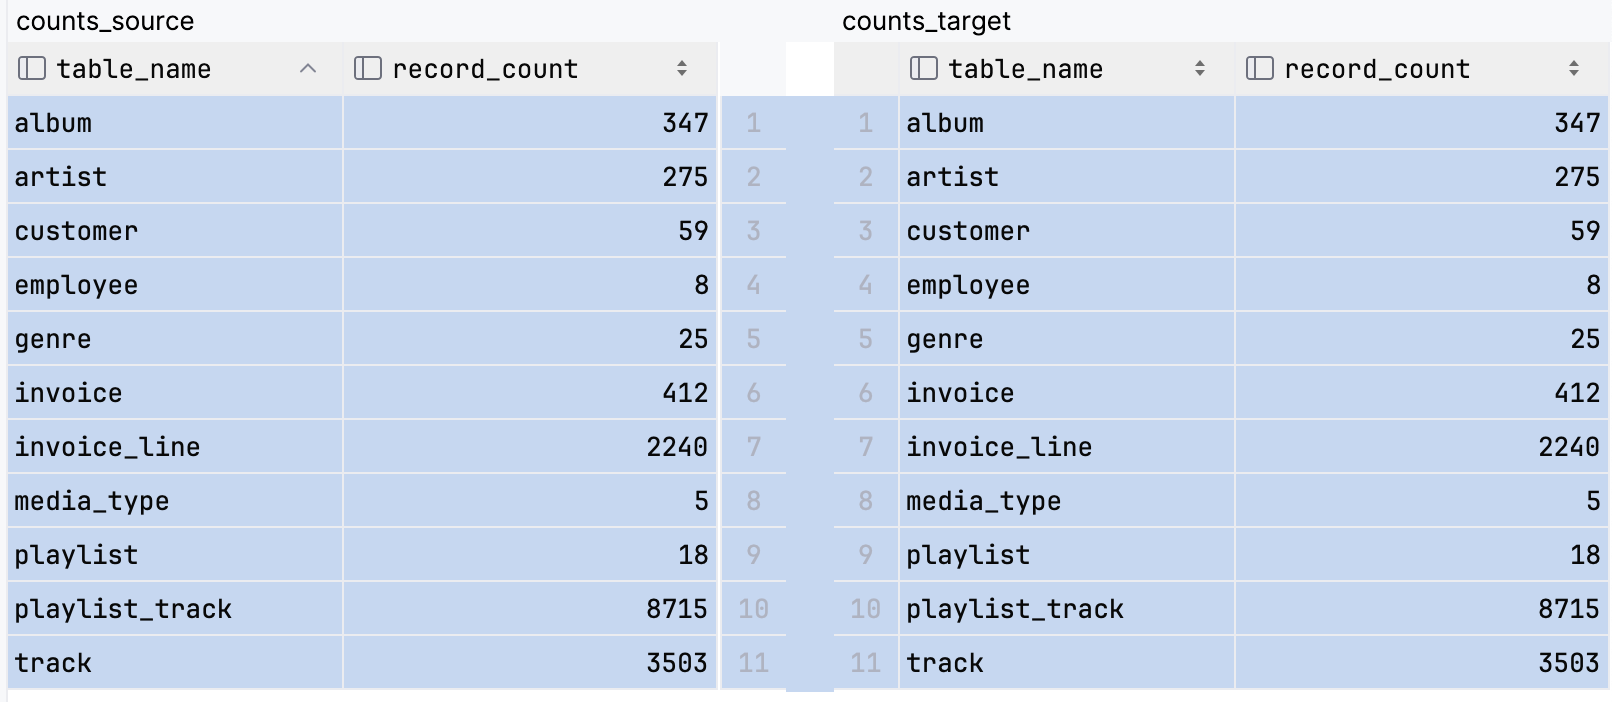
\includegraphics [scale=0.5] {my_folder/images/ex2_counts_comparering}
                  \caption{Сравнение количества строк в PostgreSQL и ClickHouse для Chinook}
                  \label{fig:ex2_counts_comparering}
                \end{figure}
                \FloatBarrier
          \item Анализ и Визуализация (Superset) \\
                ClickHouse был подключен как источник данных к Superset. На основе данных о продажах (таблица \texttt{invoice\_line}), треках (таблица \texttt{track}) и жанрах (таблица \texttt{genre}), объединенных в ClickHouse, был построен дашборд. Один из ключевых чартов на дашборде отображает количество проданных треков (или сумму продаж) в разрезе музыкальных жанров.
                \begin{figure}[h]
                  \center
                  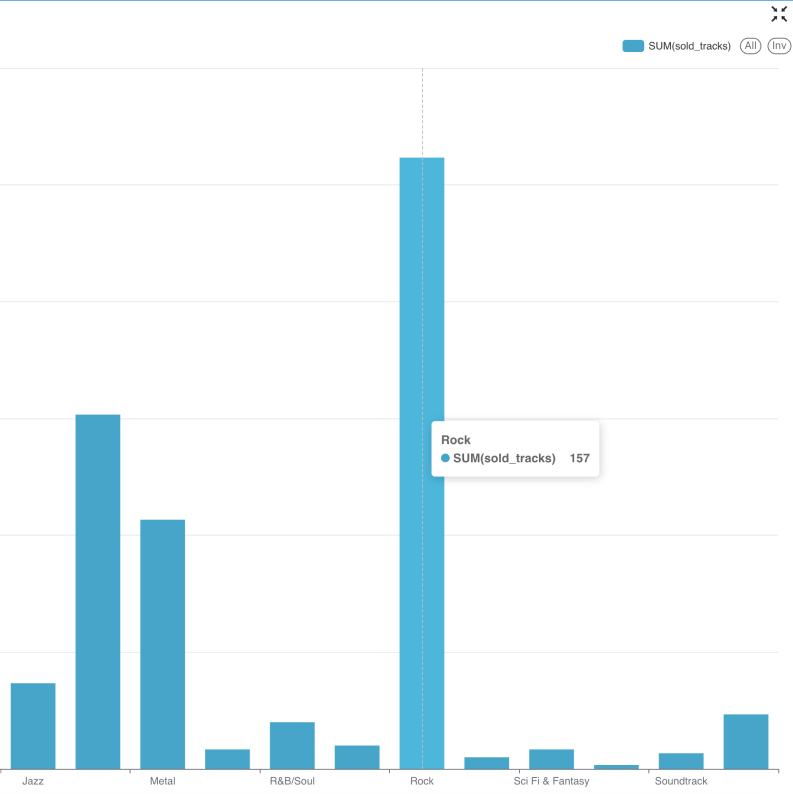
\includegraphics [scale=0.5] {my_folder/images/ex2_superset_chart}
                  \caption{Чарт в Superset "Количество продаж по жанрам"}
                  \label{fig:ex2_superset_chart}
                \end{figure}
                \FloatBarrier
        \end{itemize}
\end{enumerate}

Пример с датасетом Chinook подтверждает гибкость инструмента в развертывании платформ данных для различных сценариев. Была успешно создана инфраструктура и настроен конвейер для сбора, потоковой обработки, архивирования и аналитической обработки данных о музыкальных продажах. Финальная визуализация в Superset демонстрирует готовность платформы к решению реальных бизнес-задач по анализу данных.







% Пример ссылки на литературу \cite{avtonomova:fya,Peskov2004-ru,Kotelnikov2004-ru,Kotelnikov2004}.

%\FloatBarrier % заставить рисунки и другие подвижные (float) элементы остановиться

% \section{Выводы} \label{ch4:conclusion}

% Текст выводов по главе \thechapter.

%% Вспомогательные команды - Additional commands
%
%\newpage % принудительное начало с новой страницы, использовать только в конце раздела
%\clearpage % осуществляется пакетом <<placeins>> в пределах секций
%\newpage\leavevmode\thispagestyle{empty}\newpage % 100 % начало новой страницы